\begin{definition} \textbf{Conjunto arcoconexo.} \label{def:conjuntoconexo_simp} 
    Sea $A \subseteq \Rn{n}$. Decimos que $A$ es un conjunto \emph{arcoconexo} si para cualesquiera dos puntos $\vect{x}_0, \vect{y}_0 \in A$, existe una trayectoria continua $\gamma : [0,1] \to A$ tal que:
    \[
     \gamma(0) = \vect{x}_0 \quad \text{y} \quad \gamma(1) = \vect{y}_0.
    \]
\end{definition}
\begin{center}
        \begin{minipage}{0.45\textwidth}
            \centering
            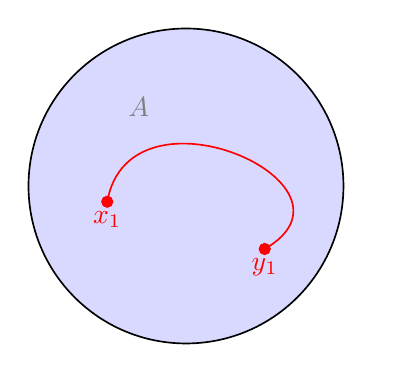
\begin{tikzpicture}
                \draw[fill=blue!15, semithick] (0,0) circle(2);
                \filldraw[red] (-1,-0.2) circle (2pt) node[below] {\(x_1\)};
                \filldraw[red] (1,-0.8) circle (2pt) node[below] {\(y_1\)};
                \draw[semithick,-,red] (-1,-0.2) to[out=80,in=30,looseness=2] (1,-0.8);
                \draw node at (-0.6,1) {\textcolor{gray}{$A$}};
            \end{tikzpicture}
        \end{minipage}
        \hspace{1cm} % espacio entre figuras
        \begin{minipage}{0.45\textwidth}
            \centering
            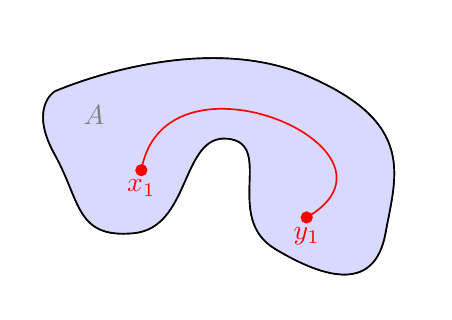
\begin{tikzpicture}
       
                % Plane R^2 on the right
               
                    \draw[semithick]
                        plot[smooth,tension=1.2] coordinates {(-0.2,0.8) (3,1) (4,-1) (2.6,-1.2)(2,0.2) (0.8,-1) (-0.2,0)(-0.2,0.8)};
                    
                    \filldraw[fill=blue!15, semithick]
                        plot[smooth, tension=1.2] coordinates {(-0.2,0.8) (3,1) (4,-1) (2.6,-1.2)(2,0.2) (0.8,-1) (-0.2,0)(-0.2,0.8)};
                        % \foreach \point in {(1,0.6), (3,0), (2.5,-1.5), (1,-1), (0.2,0.1), (1,0.6)} {
                        % \node at \point [circle,fill,inner sep=1pt] {};
                        % }
                    \filldraw[red] (0.9,-0.2) circle (2pt) node[below] {\(x_1\)};
                    \filldraw[red] (3,-0.8) circle (2pt) node[below] {\(y_1\)};
                    \draw[semithick,-,red] (0.9,-0.2) to[out=80,in=30,looseness=2] (3,-0.8);
                    \draw node at (0.3,0.5) {\textcolor{gray}{$A$}};
                    
            
            \end{tikzpicture}
        \end{minipage}
        \end{center}
        \begin{center}
        
\begin{tikzpicture}
            \node at (1.5,-2) {Conjuntos \emph{arcoconexos}};
        \end{tikzpicture}
        \end{center}

    